\documentclass[aspectratio=169]{beamer}
\useoutertheme[progressbar=frametitle]{metropolis}
\addtobeamertemplate{frametitle}{\vskip0.5ex}{}
\useinnertheme{metropolis}
\definecolor{nabgray}{rgb}{0.6,0.59,0.61}
\usecolortheme[named=nabgray]{structure}
\usepackage{tikz}
\usepackage[utf8]{inputenc}
\usepackage[portuguese]{babel}
\usepackage{fontspec}
\setmonofont{JetBrains Mono}
\setmainfont{Helvetica Neue}
\setsansfont{Helvetica Neue}
\usepackage{smartdiagram}
\usepackage{qtree}
\usepackage{verbatim}
\usepackage{svg}
\usepackage{graphicx}
\usepackage{color}
\definecolor{lightgray}{rgb}{0.95, 0.95, 0.95}
\definecolor{darkgray}{rgb}{0.4, 0.4, 0.4}
\definecolor{ocherCode}{rgb}{1, 0.5, 0} % #FF7F00 -> rgb(239, 169, 0)
\definecolor{blueCode}{rgb}{0, 0, 0.93} % #0000EE -> rgb(0, 0, 238)
\definecolor{greenCode}{rgb}{0, 0.6, 0} % #009900 -> rgb(0, 153, 0)

\usepackage{upquote}
\usepackage{listings}
\lstset{language=java,
    otherkeywords={var,record},
	% Basic design
	backgroundcolor=\color{lightgray},
	basicstyle={\small\ttfamily},
	frame=l,
	keywordstyle=\footnotesize\color{blue},
	escapeinside={<@}{@>},
	breaklines=true,
	% Line numbers
	xleftmargin={0.75cm},
	numbers=left,
	stepnumber=1,
	firstnumber=1,
	numberfirstline=true
	% Code design
	identifierstyle=\color{black},
	keywordstyle=\color{ocherCode}\bfseries,
	ndkeywordstyle=\color{greenCode}\bfseries,
	stringstyle=\color{ocherCode}\ttfamily,
	commentstyle=\color{darkgray}\ttfamily,
	tabsize=2,
	showtabs=true,
	showspaces=false,
	showstringspaces=false,
	extendedchars=true,
	breaklines=true
}

\lstdefinelanguage{bash}{
    basicstyle=\ttfamily,
    showstringspaces=false,
    commentstyle=\color{red},
    keywordstyle=\color{blue},
    numbers=right,
    xleftmargin={0.25cm}
}

\usebackgroundtemplate
{
	\includegraphics[width=\paperwidth]{Images/contenido}%
}


\title{Do clickops para IaC warm standby, alta disponibilidade multiregião com OpenTofu e Kubernetes}
\author{Víctor Orozco - @tuxtor}
\institute{Nabenik}
\date{19 de setembro de 2024}

\begin{document}

{
    \usebackgroundtemplate{
\includegraphics[width=\paperwidth]{Images/portada}}
    \setbeamercolor{frametitle}{fg=red}
    \usebeamercolor[fg]{normal text}
    \frame{\titlepage}
}

\begin{frame}{Introdução}
	\begin{itemize}
	\item \textbf{Objetivo da Palestra}:
	\begin{itemize}
		\item Conversar acerca da transformação de uma infraestrutura  "clickops" para DR Warm Standby.
		\item Explicar como essa transformação ajudou a atingir um SLA de 99\%.
	\end{itemize}
	\item \textbf{Visão geral dos tópicos}:
	\begin{itemize}
		\item O problema
		\item A solução
		\item Ideias importantes
	\end{itemize}
\end{itemize}
\end{frame}



{
	\usebackgroundtemplate{
\includegraphics[width=\paperwidth]{Images/separador}}
	\setbeamercolor{normal text}{fg=white}
	\setbeamercolor{frametitle}{fg=red}
	\usebeamercolor[fg]{normal text}
	\section{O problema}
}


%\begin{frame}{A plataforma}
%	\begin{exampleblock}{IDP}
%		IDP é um software de delivery (rotas, pacotes, GPS, tracking, real time) corporativo. Ele recebe pedidos de aplicativos e permite que gestores planifiquem rotas de delivery.\\
%	\end{exampleblock}
%	\begin{exampleblock}{IDP}		
%		A plataforma é um backend corporativo que recebe pedidos de outras plataformas.
%	\end{exampleblock}
	
%\end{frame}

\begin{frame}
	\begin{figure}
		\centering
		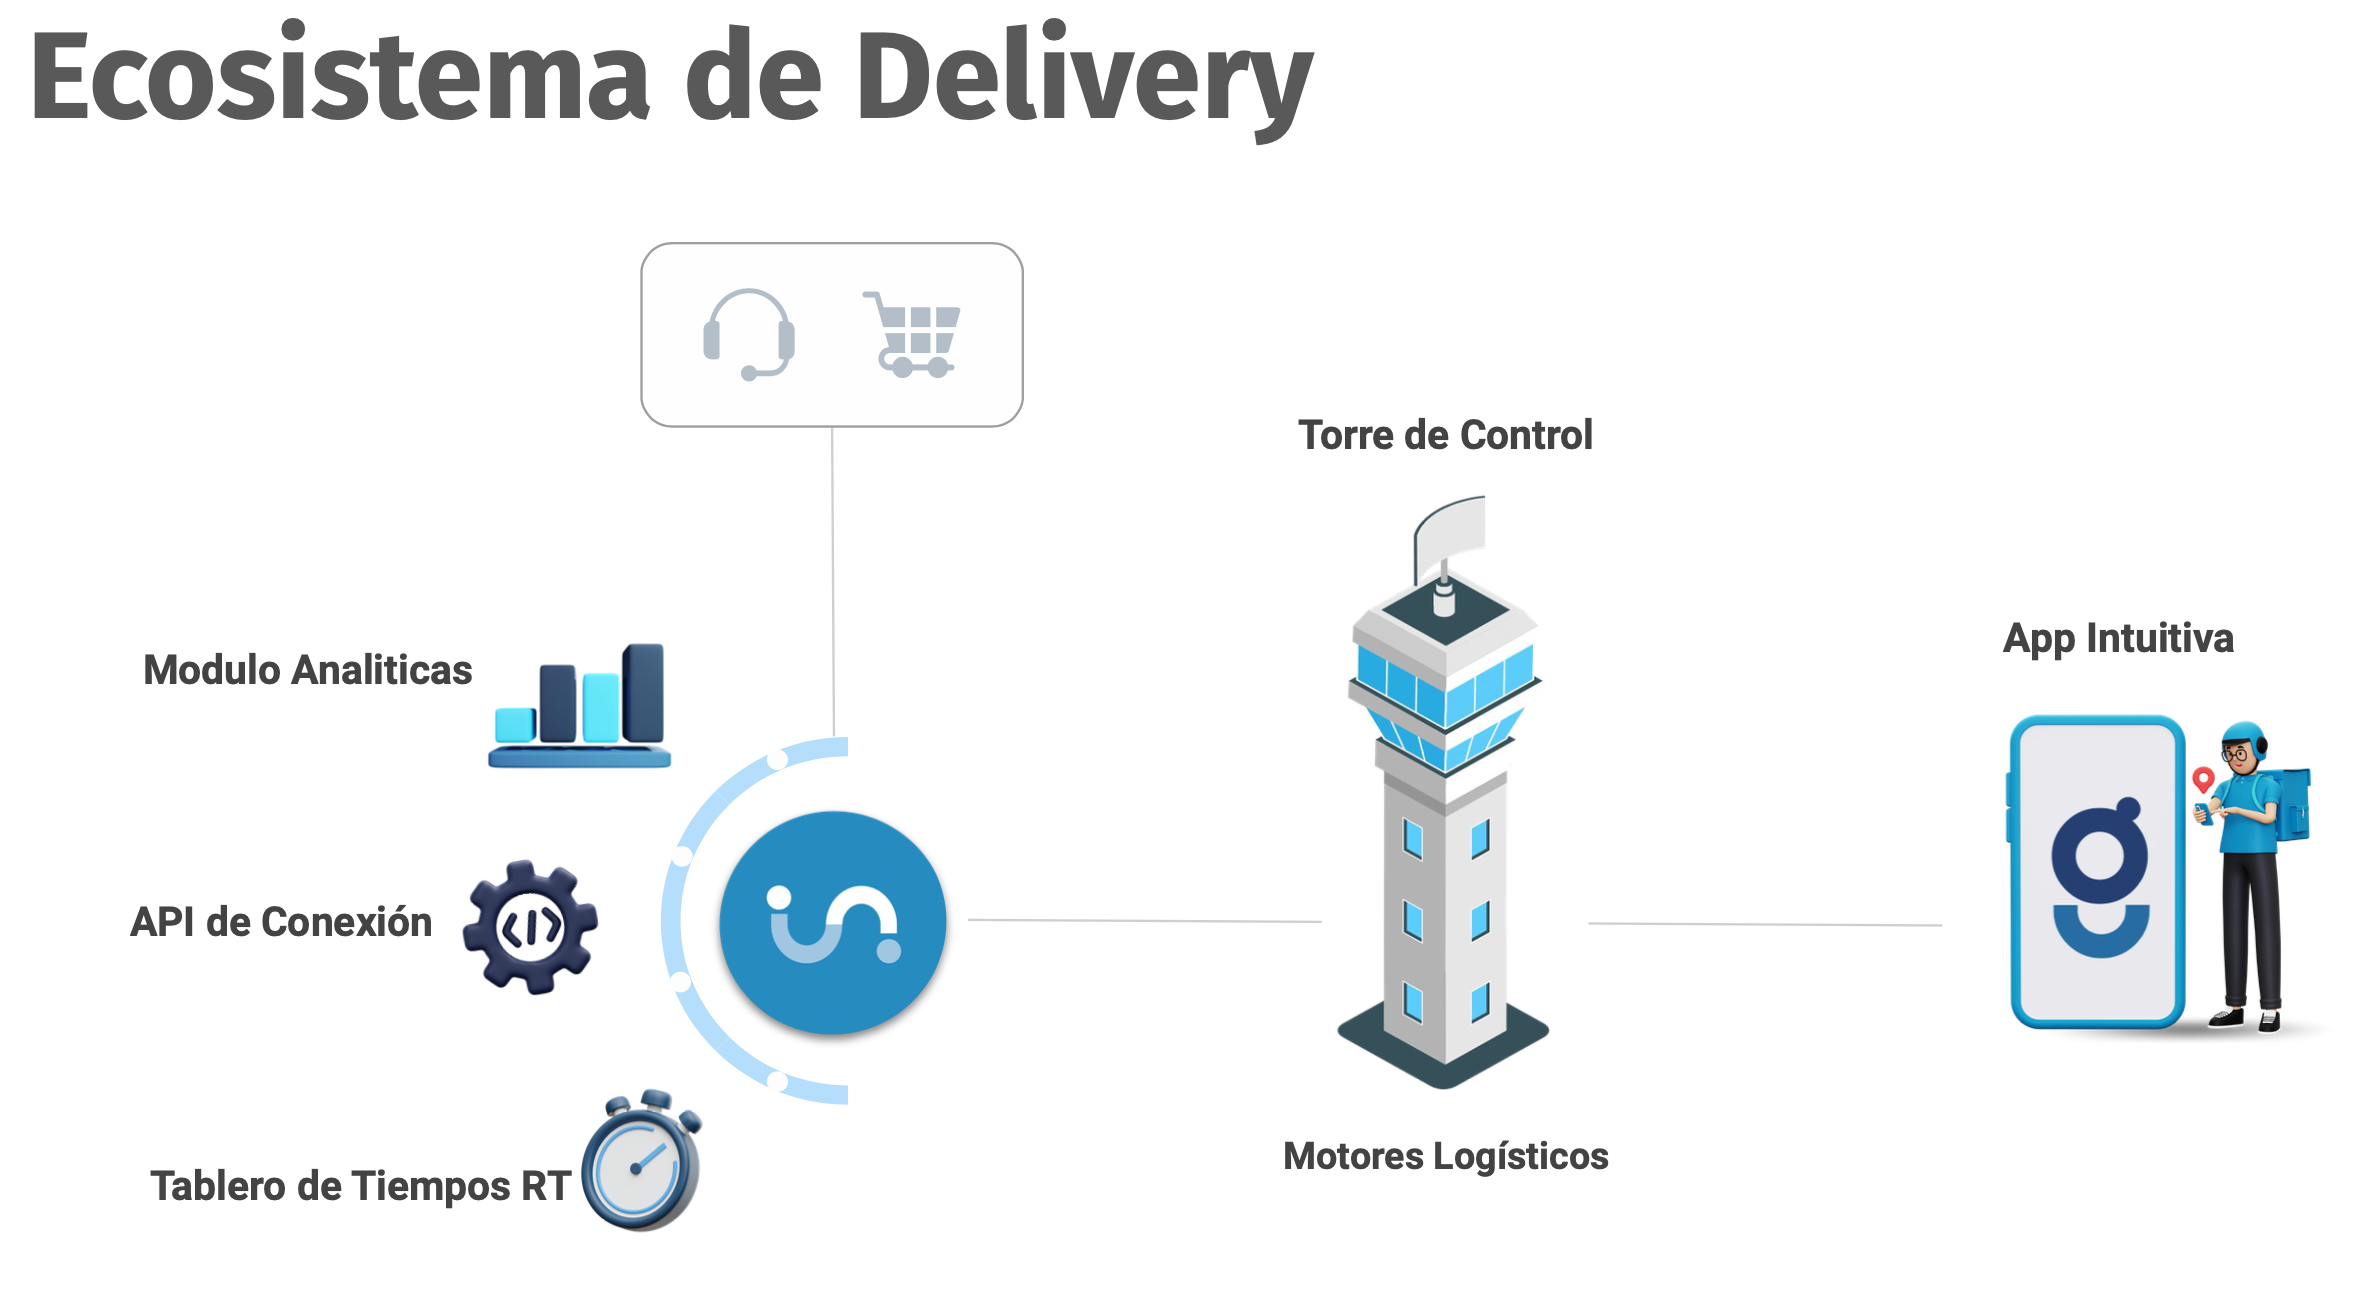
\includegraphics[width=\linewidth]{Images/ecosistema}
	\end{figure}
\end{frame}

\begin{frame}
	\begin{figure}
		\centering
		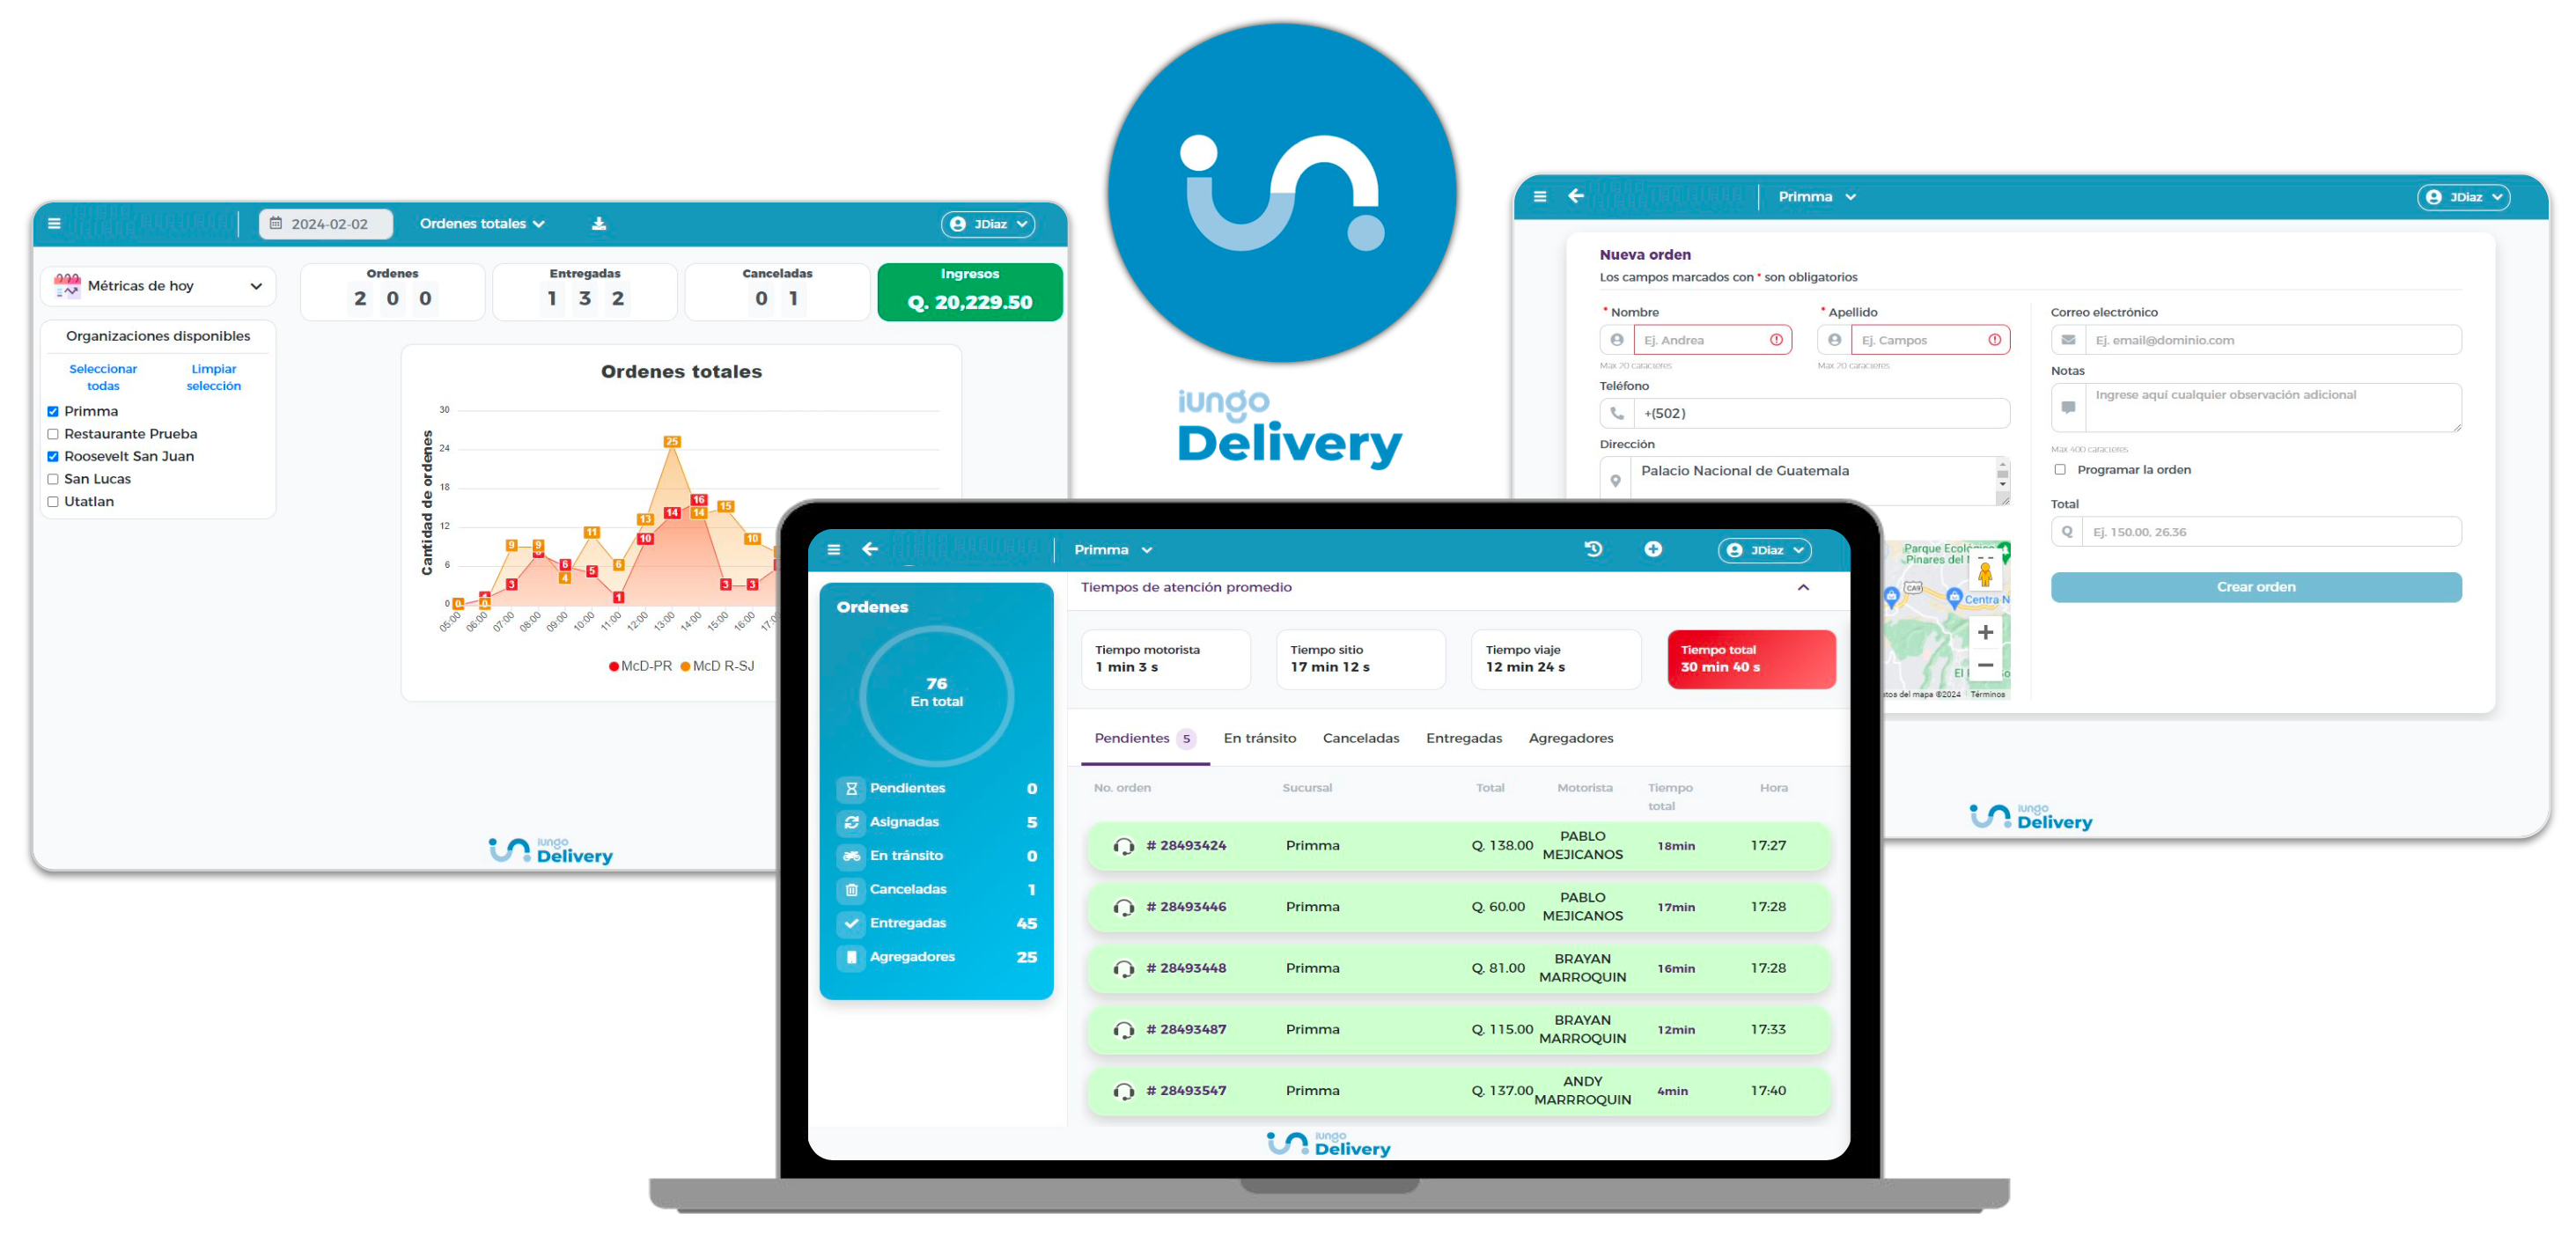
\includegraphics[width=\linewidth]{Images/dashboard}
	\end{figure}
\end{frame}



\begin{frame}{O problema}
IDP v1
	\begin{itemize}		
		\item A Iungo (dona do software) cria projetos de inovação digital em modalidade Lean
		\item Infraestrutura lean = Clickops
	\end{itemize}
IDP v2
	\begin{itemize}		
	\item \textbf{Mais clientes = SLA 99\%}
	\item A infraestrutura lean estava ficando limitada
	\item 1\% = 432 minutos = 7 horas por mês
\end{itemize}
\end{frame}



\begin{frame}{¿O que é ``Clickops''?}
	
	\begin{exampleblock}{Definição}
		Gerenciamento manual da infraestrutura via console -e.g. AWS Console, OCI console-.
	\end{exampleblock}
		\begin{itemize}		
		\item \textbf{Desvantagens}:
		\begin{itemize}
			\item Falta de consistência (multi A-Z)
			\item \textbf{Falta de homologação (multirregião)}
			\item Risco de erros humanos
			\item SREs mudam, é a vida
			\item Auditorias são complicadas com Runbooks
		\end{itemize}
		\end{itemize}
\end{frame}


\begin{frame}
\begin{figure}
	\centering
	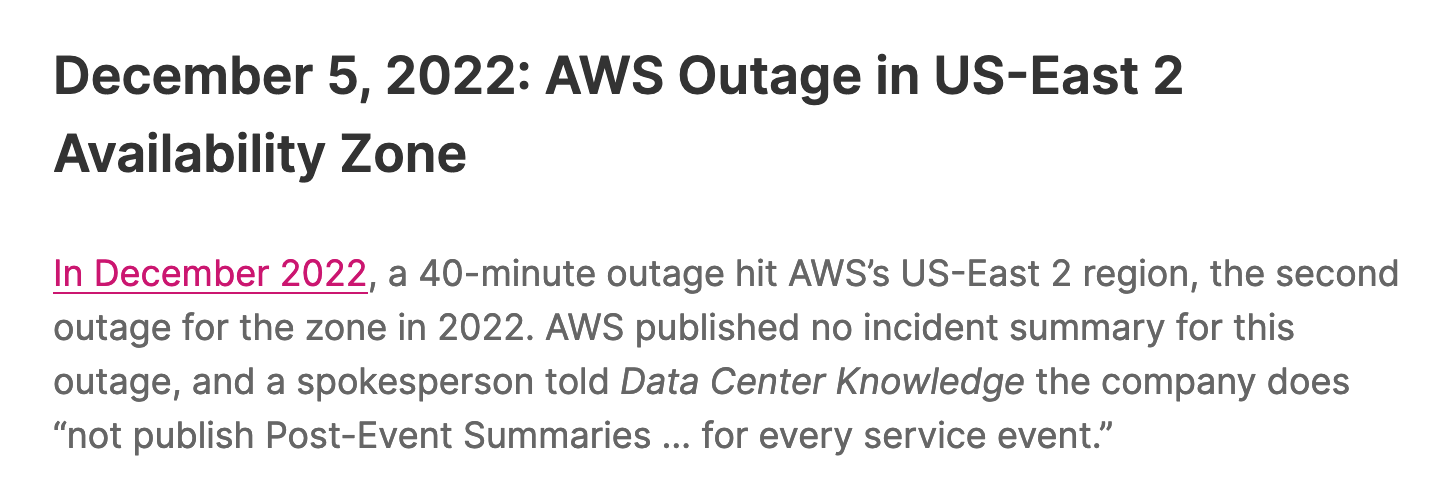
\includegraphics[width=0.7\linewidth]{Images/awsoutage}
	\caption{AWS Outage}
	\label{fig:awsoutage}
\end{figure}
https://www.datacenterknowledge.com/outages/a-history-of-aws-cloud-and-data-center-outages
\end{frame}

\begin{frame}
\begin{figure}
	\centering
	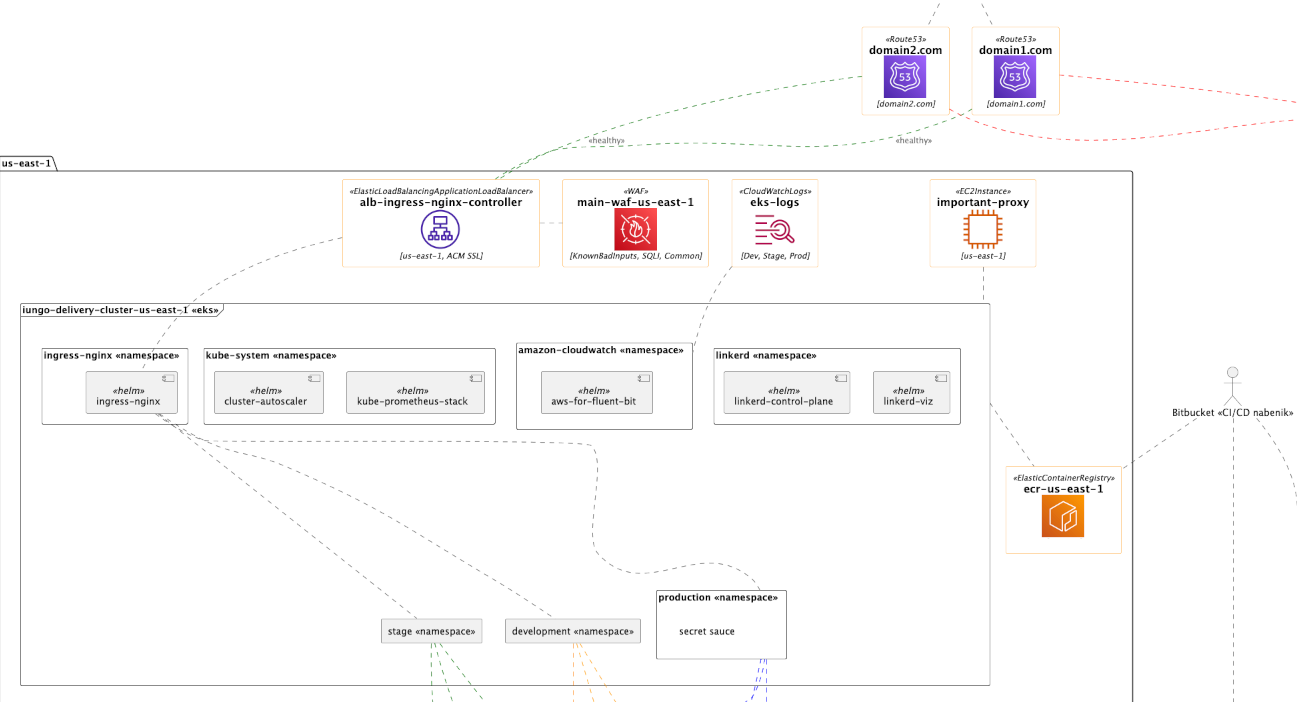
\includegraphics[width=\linewidth]{Images/problema}

\end{figure}
\end{frame}


{
	\usebackgroundtemplate{
\includegraphics[width=\paperwidth]{Images/separador}}
	\setbeamercolor{normal text}{fg=white}
	\setbeamercolor{frametitle}{fg=red}
	\usebeamercolor[fg]{normal text}
	\section{A solução}
}


\begin{frame}{Warm Standby}
\begin{figure}
	\centering
	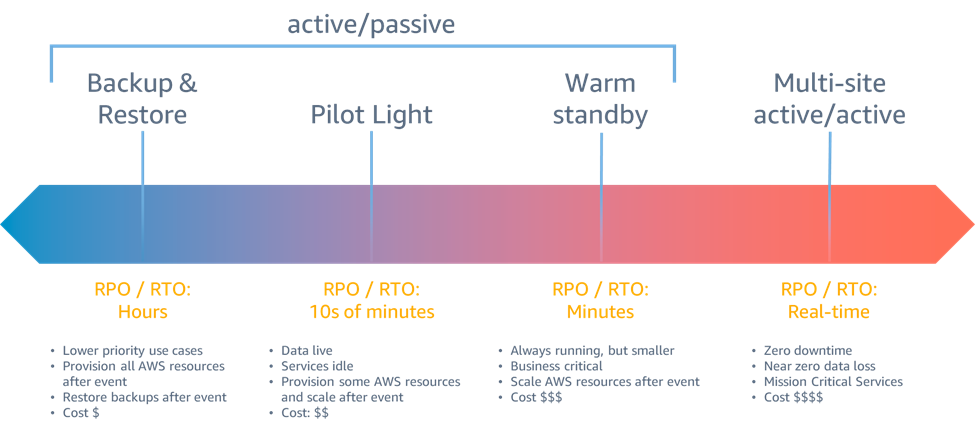
\includegraphics[width=0.9\linewidth]{Images/warmsandby}
	\caption{Disaster recovery strategies}
	\label{fig:warmsandby}
\end{figure}
https://docs.aws.amazon.com/whitepapers/latest/disaster-recovery-workloads-on-aws/disaster-recovery-options-in-the-cloud.html
\end{frame}

\begin{frame}{Warm Standby}
	\begin{itemize}
		\item \textbf{Visão Geral do DR Warm Standby}:
		\begin{itemize}
			\item Infraestrutura (reduzida) pronta para failover.
			\item Capacidade de recuperação rápida.
			\item Multi A-Z
		\end{itemize}
				\item \textbf{Desafios com o ``Clickops"}:
		\begin{itemize}
			\item Sem recuperação rápida
			\item Impossível criar a parte WARM sem errar
			\item Os aplicativos estavam prontos para IaC, mas a infraestrutura não
		\end{itemize}
	\end{itemize}
\end{frame}

\begin{frame}{Warm Standby}
\begin{figure}
	\centering
	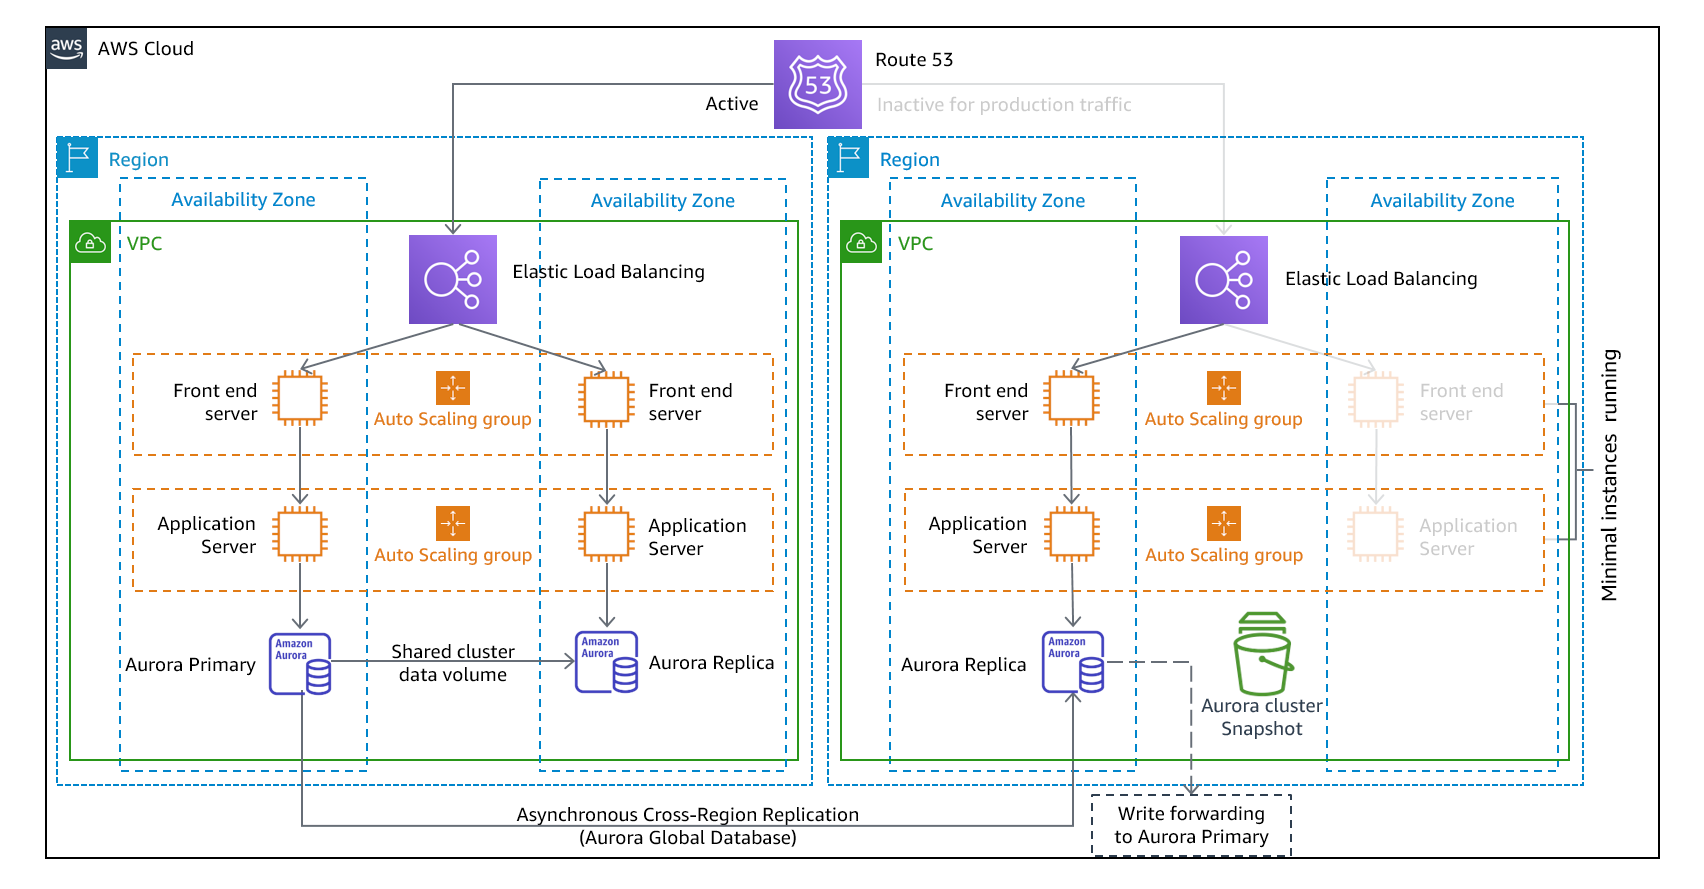
\includegraphics[width=0.8\linewidth]{Images/warmsandbyaws}
	\caption{Warm Standby}
	\label{fig:warmsandbyaws}
\end{figure}
https://docs.aws.amazon.com/whitepapers/latest/disaster-recovery-workloads-on-aws/disaster-recovery-options-in-the-cloud.html
\end{frame}




{
	\usebackgroundtemplate{
\includegraphics[width=\paperwidth]{Images/separador}}
	\setbeamercolor{normal text}{fg=white}
	\setbeamercolor{frametitle}{fg=red}
	\usebeamercolor[fg]{normal text}
	\section{Ideias importantes}
}

\begin{frame}{Ideia 0: Seja cloud native sempre}
	TL;DR: Um bom chassis de microserviço facilita tudo\\
	
	Na capa de aplicativos, precisamos reconfigurar os pipelines, {\LARGE só!}
	\begin{figure}
		\centering
		
\includegraphics[width=\linewidth]{Images/commits}
	\end{figure}
	
	
\end{frame}

\begin{frame}{Ideia 0: Seja cloud native sempre}
\textbf{Backend:} Java (Quarkus) + Eclipse JKube
			\begin{enumerate}
			\item Codebase: Github Flow
			\item Dependencies: Maven
			\item Config: MicroProfile Config, Vault
			\item Backing services: Kafka (SmallRye Reactive Messaging), JPA + Hibernate Panache, MicroProfile Config
			\item Build, release, run: Maven, Eclipse JKube
			\item Processes: JAX-RS, MicroProfile Rest Client
		\end{enumerate}
\end{frame}

\begin{frame}{Ideia 0: Seja cloud native sempre}
\textbf{Backend:} Java (Quarkus) + Eclipse JKube
		\begin{enumerate}
			\item Port Binding: Kubernetes + MicroProfile Config
			\item Concurrency: HPA + MicroProfile Health + MIcroProfile Metrics
			\item Disposability: Supersonic and subatomic (Quarkus)
			\item Dev/prod parity: Maven profile + Quarkus Profiles + MicroProfile Config
			\item Logs: ElasticSearch Operator
			\item Admin processes: Flyway
		\end{enumerate}
\end{frame}

\begin{frame}{Ideia 0: Seja cloud native sempre}
\textbf{Frotend:} TypeScript (Angular) + Kustomize
		\begin{enumerate}
			\item Codebase: Github Flow
			\item Dependencies: NPM
			\item Config: Angular Profiles
			\item Backing services: Ingress, ALB
			\item Build, release, run: NPM, Kustomize
			\item Processes: Container NGINX
		\end{enumerate}

\end{frame}

\begin{frame}{Ideia 0: Seja cloud native sempre}
 \textbf{Backend:} TypeScript (Angular) + Kustomize
		\begin{enumerate}
			\item Port Binding: Kubernetes + Angular Profiles + Pipelines
			\item Concurrency: HPA + Kubernetes Operator + Linkerd
			\item Disposability: Nginx
			\item Dev/prod parity: Angular Profile
			\item Logs: ElasticSearch Operator
			\item Admin processes: N/A
		\end{enumerate}
\end{frame}


\begin{frame}{Ideia 1: Separar os ciclos de vida}
	
	\begin{itemize}
		\item \textbf{1. Infraestrutura - Não muda frequentemente - OpenTofu}:
		\begin{itemize}
			\item Infraestrutura cloud
			\item Kubernetes operators
			\item Secret vaults
		\end{itemize}
		\item \textbf{2. Aplicativos - Muda constantemente - CI/CD}:
		\begin{itemize}
			\item Java - JKube
			\item JavaScript - Kustomize
			\item CI/CD Bitbucket, single source of truth
			\item Um pipeline, duas AZ
			\item AWS AutoScaler + HPA = Infraestrutura reducida!
		\end{itemize}
	\end{itemize}
\end{frame}


\begin{frame}{Ideia 1: Separar os ciclos de vida}
	
	\begin{columns}[T] % contents are top vertically aligned
		
		\begin{column}[T]{10cm} % alternative top-align that's better for graphics

\textbf{Opções}:
	\begin{itemize}
		\item Terraform
		\item \textbf{Opentofu}
		\item Cloudformation (AWS)
		\item Pulumi
		\item Serverless Framework
	\end{itemize}
\textbf{OpenTofu}:
	\begin{itemize}
		\item Gestão e provisionamento da infraestrutura
		\item Deploy automatizado
		\item \textbf{Feature parity com Terraform mas ainda falta documentação}
	\end{itemize}
		\end{column}
		\begin{column}[T]{5cm} % each column can also be its own environment
			\begin{figure}
			\centering
			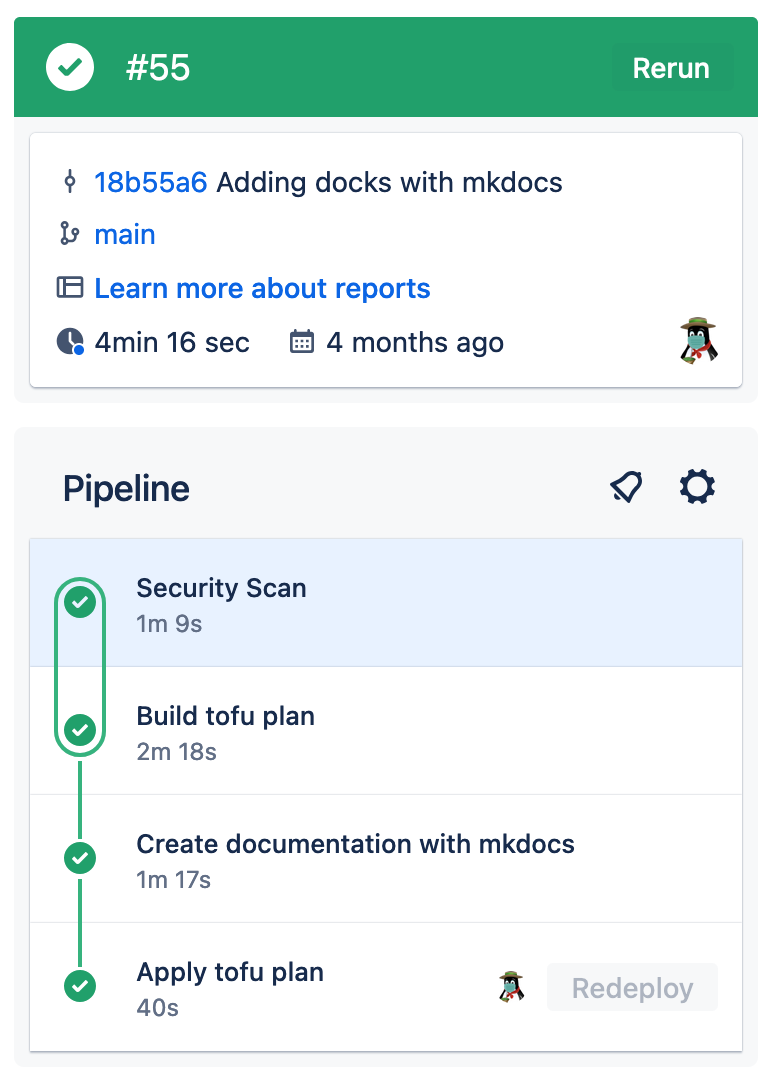
\includegraphics[width=\linewidth]{Images/tofupipeline}
		\end{figure}
		
		\end{column}
	\end{columns}
	

	
\end{frame}

\begin{frame}{Ideia 2: Diferenciar compartilhado vs. global}
Os módulos do HCL são nossos amigos, bem planejados eles podem ser reutilizados
	
	\begin{columns}[T] % contents are top vertically aligned
		
		\begin{column}[T]{5cm} % alternative top-align that's better for graphics
		
		\begin{itemize}
			\item \textbf{Recursos globais:} IAM, Route53, Cloudfront
			\item \textbf{Recursos regionais:} EKS, ECR, EC2, MKS, CloudWatch
			\item \textbf{Especial:} RDS replication
		\end{itemize}
		\end{column}
		\begin{column}[T]{5cm} % each column can also be its own environment
				\begin{figure}
				\centering
				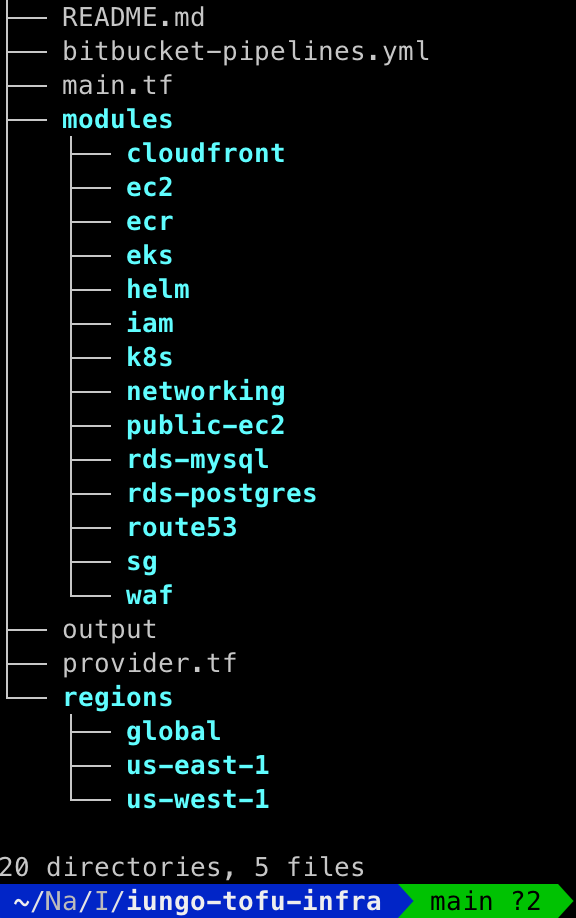
\includegraphics[width=0.9\linewidth]{Images/tofu}
				
			\end{figure}
		\end{column}
	\end{columns}
	
\end{frame}


\begin{frame}

			\begin{figure}
				\centering
				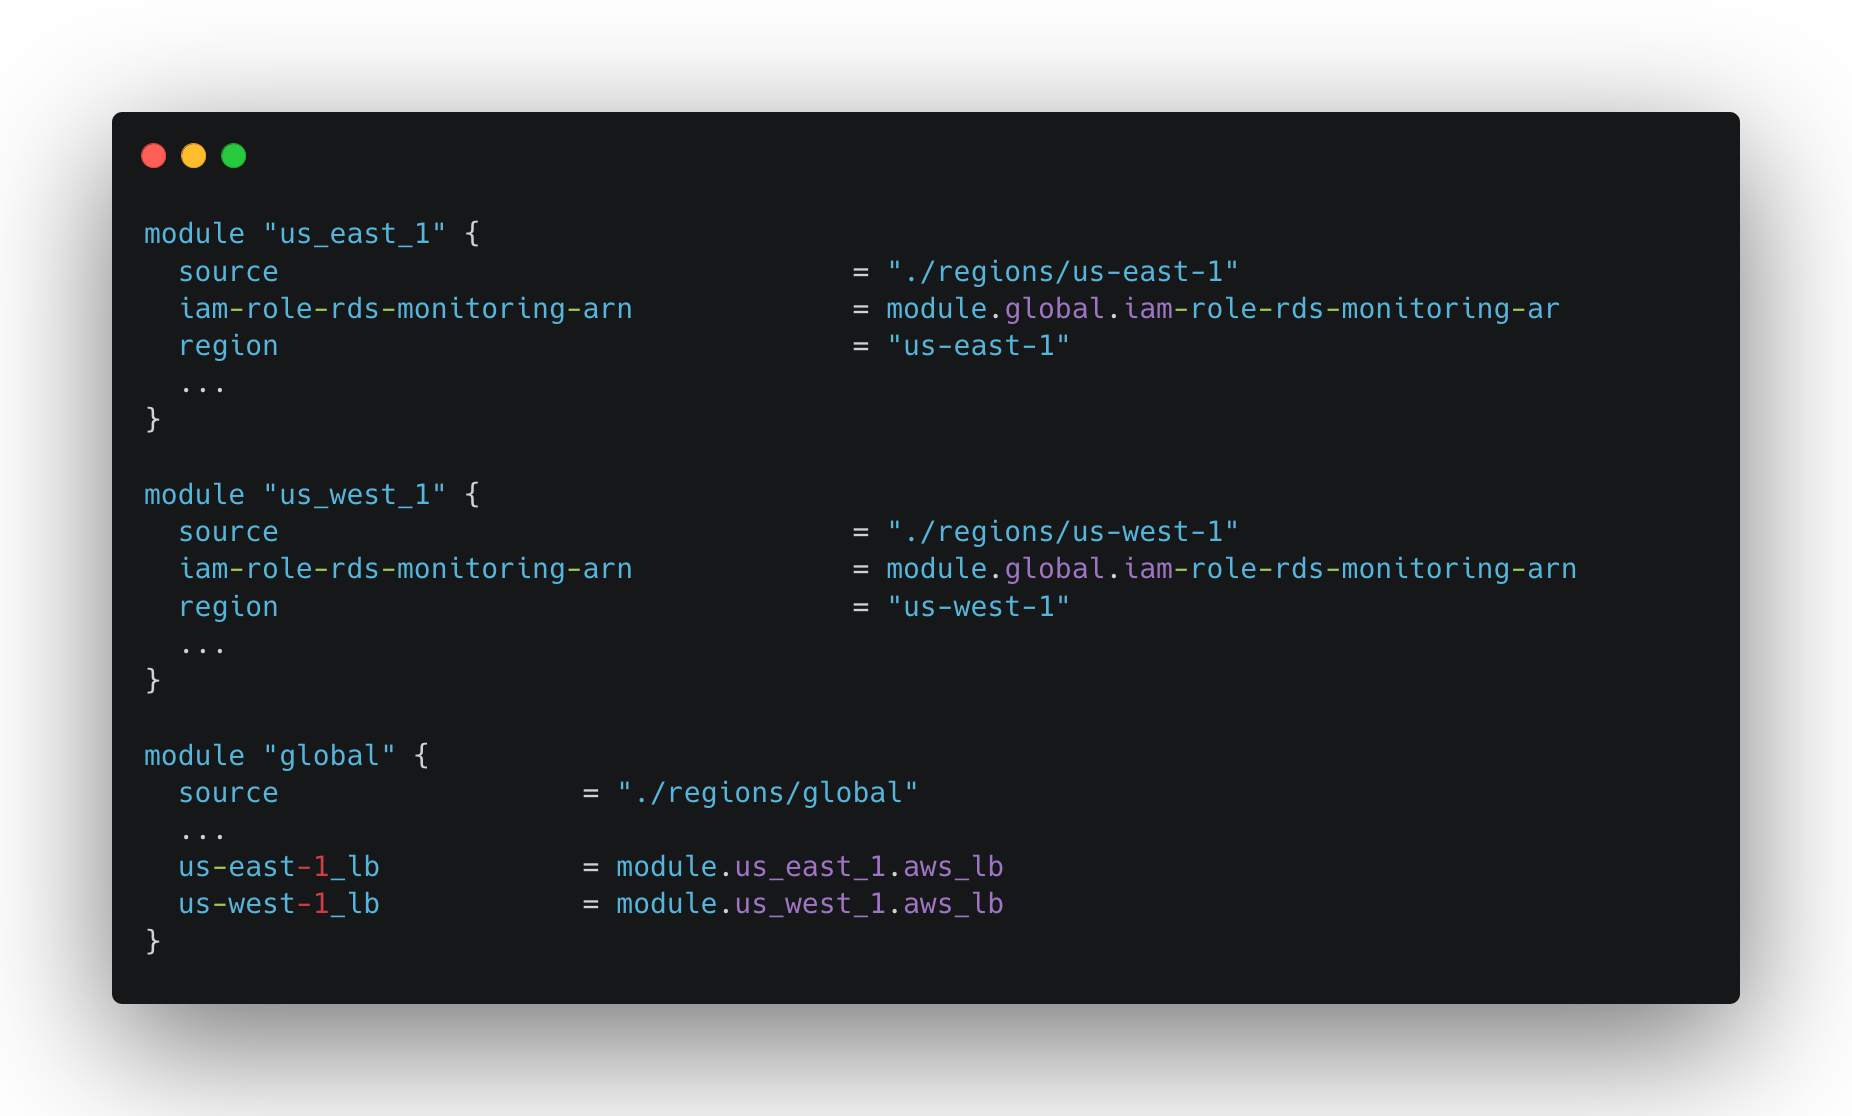
\includegraphics[width=0.9\linewidth]{Images/hcl}
				
			\end{figure}
	
\end{frame}


\begin{frame}
	
	
	\begin{figure}
		\centering
		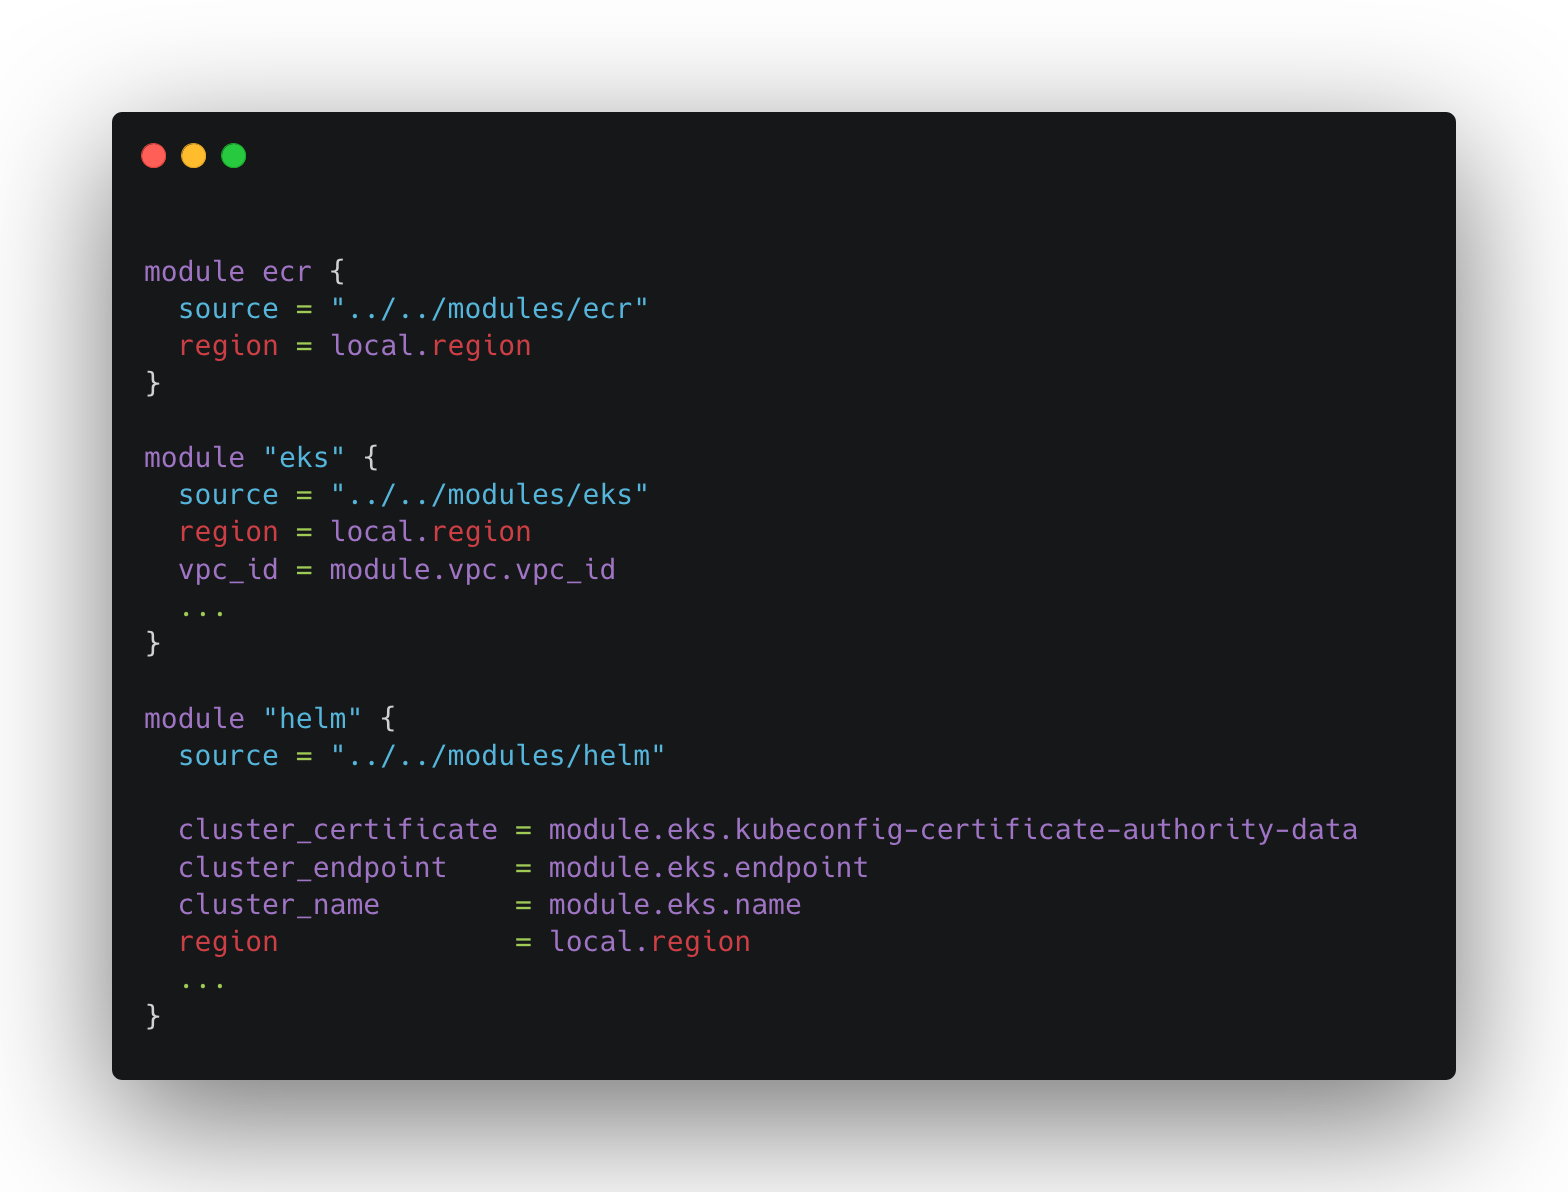
\includegraphics[width=0.7\linewidth]{Images/modulos}
		\caption{regions/us-east-1.tf}
	\end{figure}
	
\end{frame}


\begin{frame}{Resultados}
	\begin{itemize}
		\item \textbf{Melhoria no SLA}:
		\begin{itemize}
			\item 99.00\% uptime atingido e resiliência testada
		\end{itemize}
		\item \textbf{Redução de riscos e erros}:
		\begin{itemize}
			\item Menos erros manuais.
			\item Redução de riscos operacionais.
		\end{itemize}
		\item \textbf{Maior eficiência operacional}:
		\begin{itemize}
			\item Deploys mais rápidos.
			\item Menos esforço manual.
		\end{itemize}
		\item \textbf{Preparação para o Futuro}:
		\begin{itemize}
			\item Suporte a crescimento e novas demandas.
		\end{itemize}
	\end{itemize}
\end{frame}


\begin{frame}
	
	\begin{figure}
		\centering
		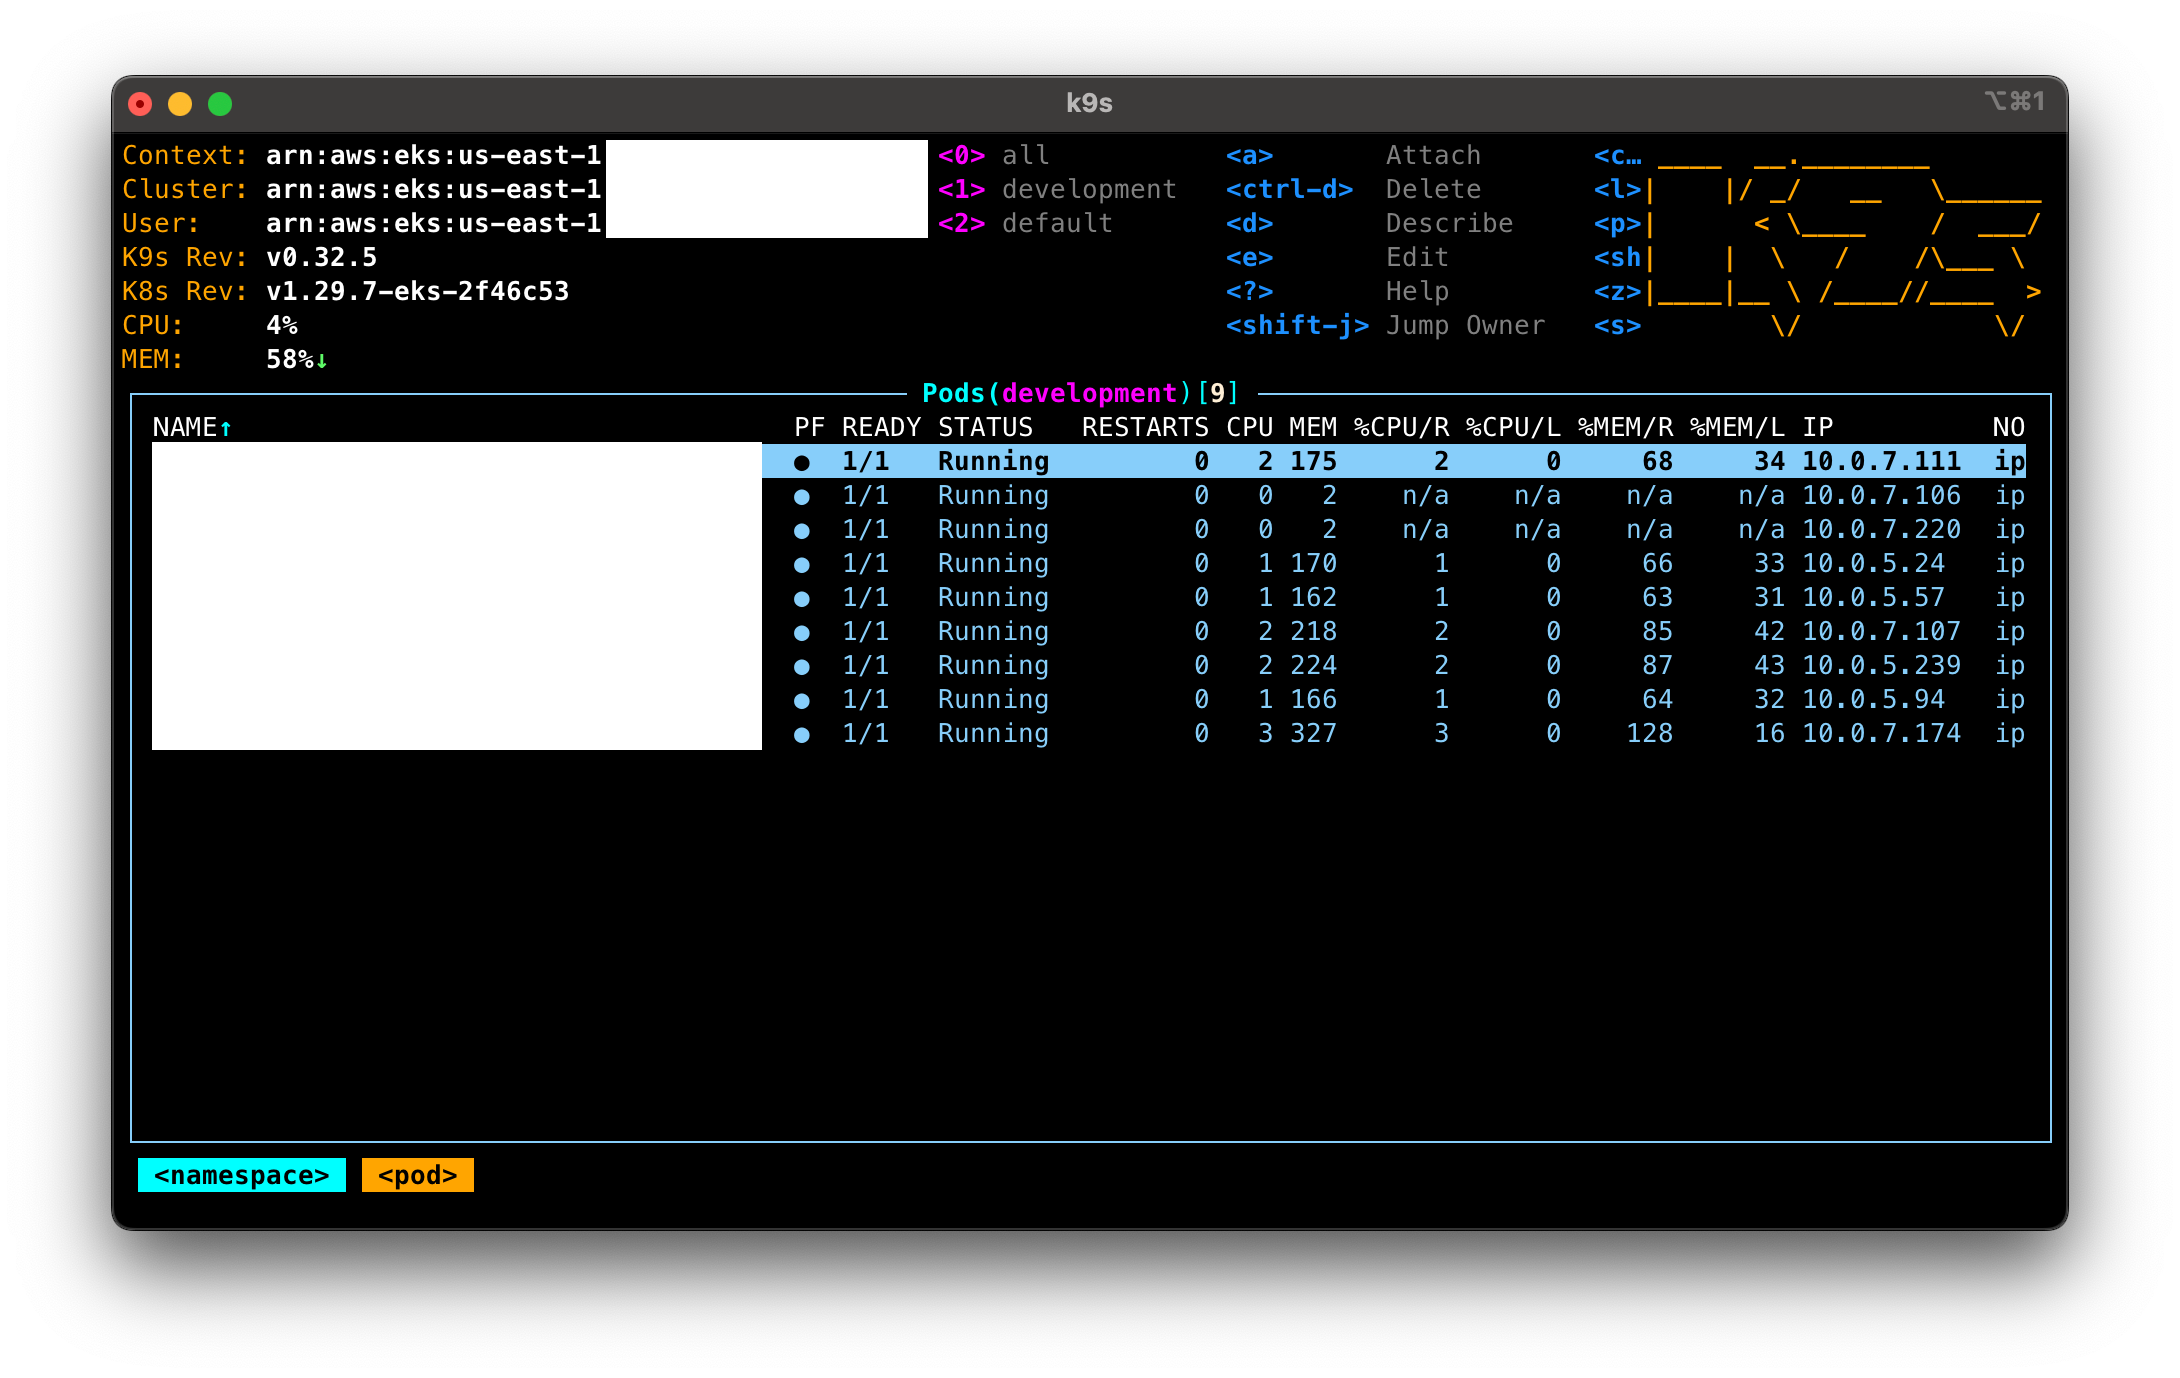
\includegraphics[width=0.9\linewidth]{Images/east}
		
	\end{figure}
	
\end{frame}

\begin{frame}{Perguntas}
	\centering
	\textbf{\Large Perguntas?}
\end{frame}


\begin{frame}{Víctor Orozco}
	\begin{columns}[T] % contents are top vertically aligned
		
		\begin{column}[T]{4cm} % alternative top-align that's better for graphics
			\begin{figure}
				\centering
				
\includegraphics[width=0.8\linewidth]{Images/logos}
			\end{figure}
		\end{column}
		\begin{column}[T]{6cm} % each column can also be its own environment
			\begin{itemize}
				\item vorozco@nabenik.com
				\item \href{https://twitter.com/tuxtor}{@tuxtor}
				\item \href{https://vorozco.com}{https://vorozco.com}
				\item \href{https://tuxtor.shekalug.org}{https://tuxtor.shekalug.org}
			\end{itemize}
			\begin{center}
				
\includegraphics[width=0.1\linewidth]{Images/cclogo}
				\\
				This work is licensed under Creative Commons Attribution-NonCommercial-ShareAlike 3.0 Guatemala (CC BY-NC-SA 3.0 GT).
			\end{center}
		\end{column}
	\end{columns}
\end{frame}



\end{document}

